% !TEX root = ../agglo_clust_review.tex
% 
\begin{figure}
\centering

        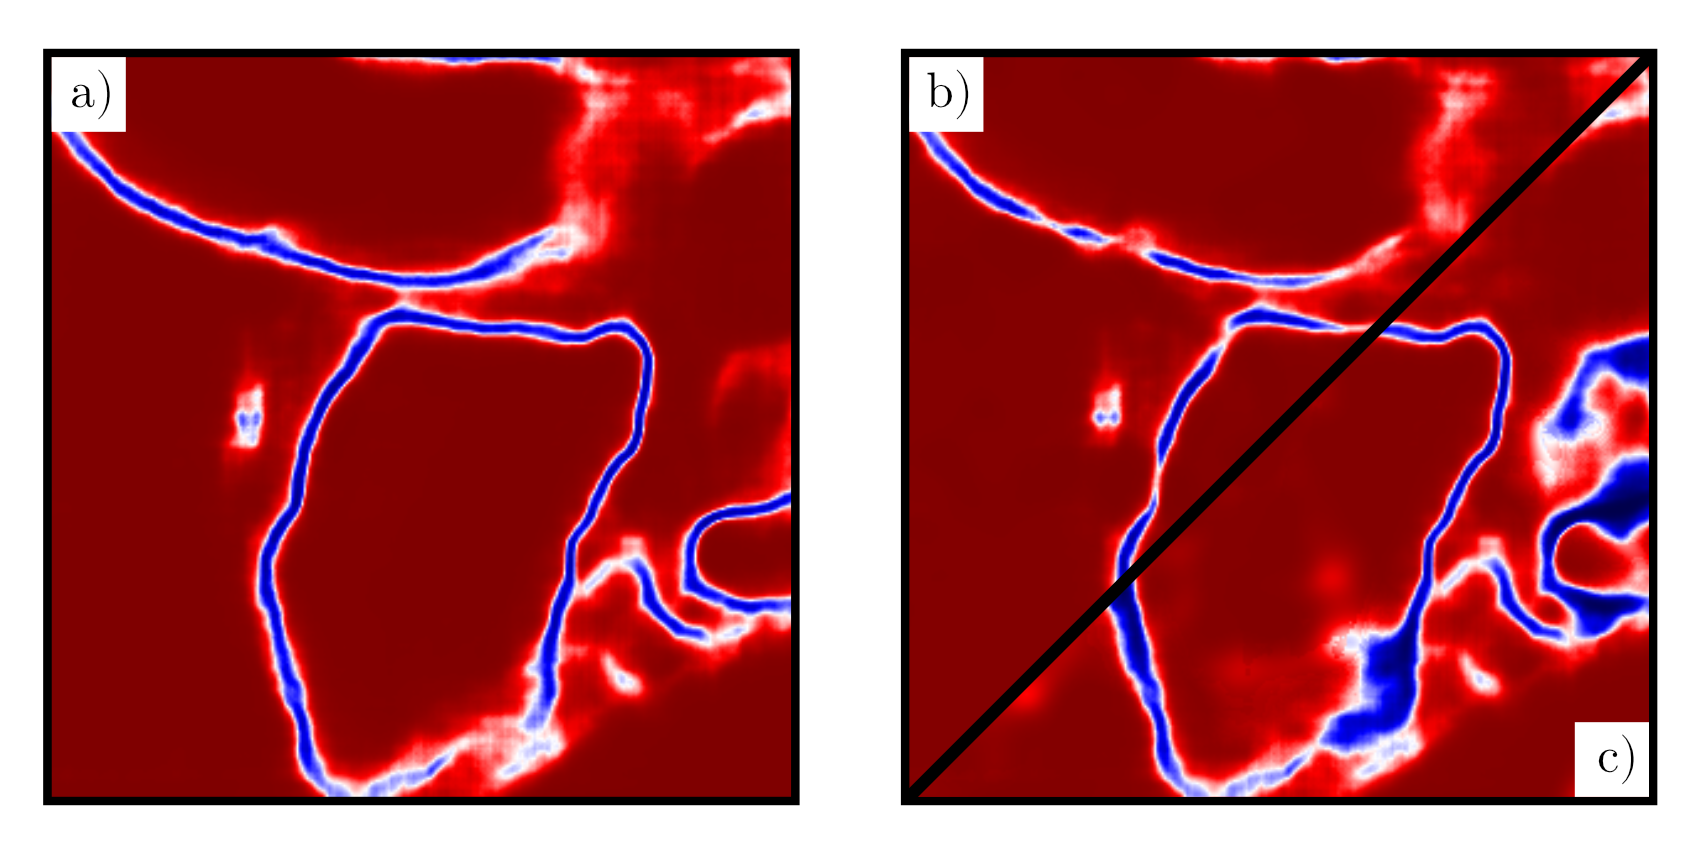
\includegraphics[width=0.48\textwidth,trim=0.1in 0.0in 0.05in 0.0in,clip]{figs/noisy_affs_comparison.png}
   
    \caption{The two figures represent the predictions of the CNN a) without added noise, b) with the addition of the merge-biased noise defined in Eq. \ref{eq:opensimplex_noise_def} and c) with split-biased noise. The color of each pixel represents how probable it is for it to be in the same cluster with its neighboring pixel on the right (red: same cluster; blue: different ones). Adding merge-biased noise tends to create holes in the boundaries; split-biased noise add non-existing boundaries \TODO{Add colorbar?}}
    % \label{fig:isbi-examples}
\end{figure}% 

\begin{figure*}
\centering
        \begin{subfigure}[t]{0.48 \textwidth}
        \centering
        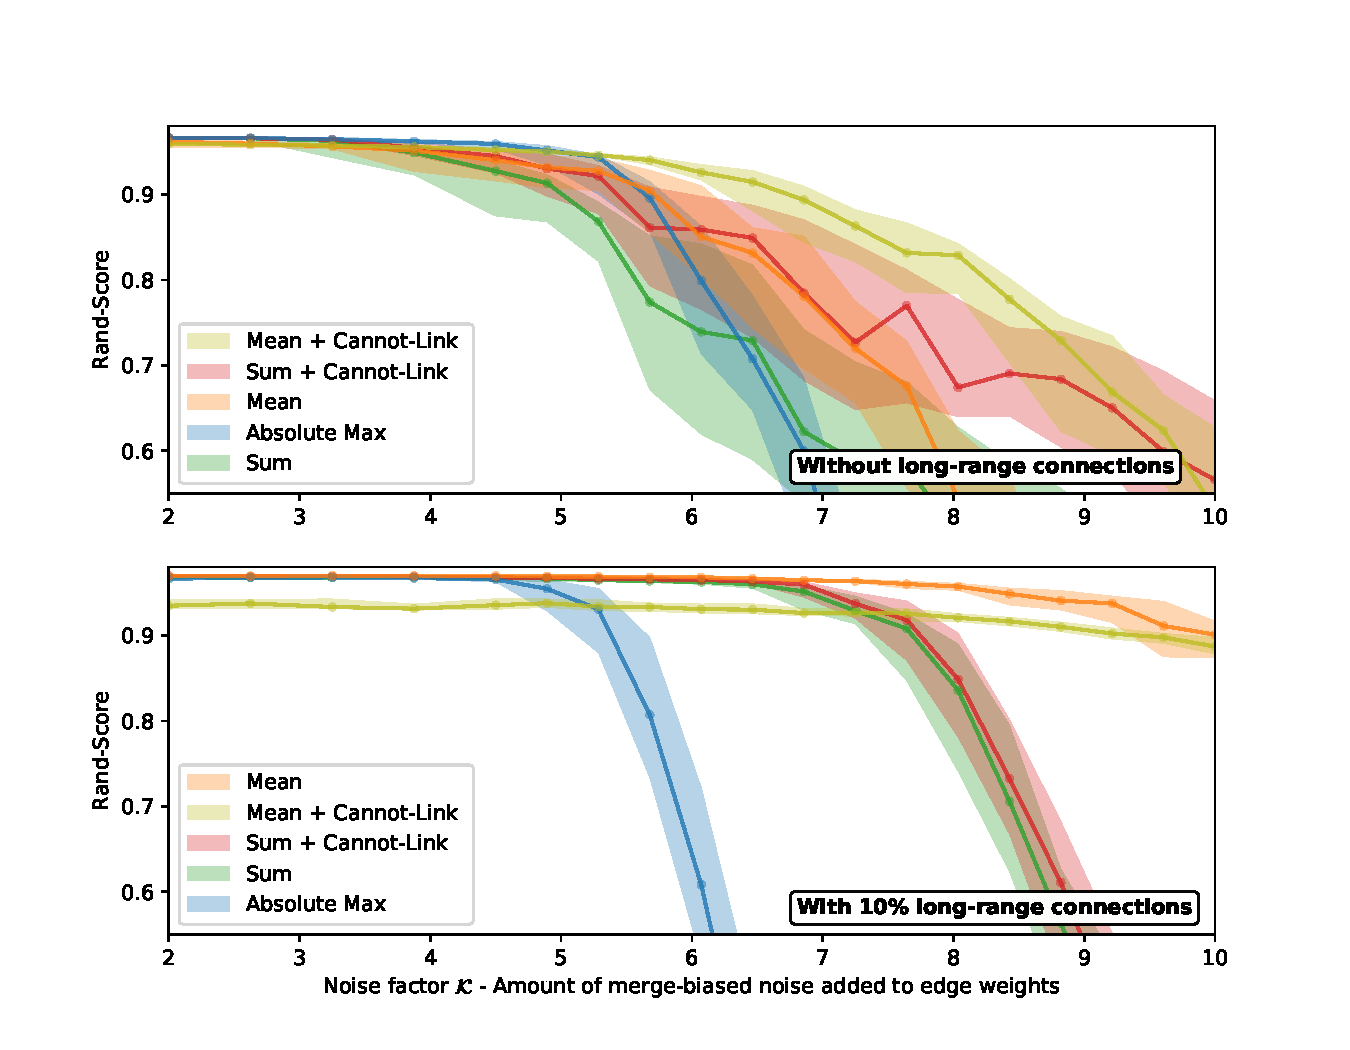
\includegraphics[width=0.98\textwidth,trim=0.35in 0.35in 0.35in 0.35in,clip]{./figs/merge_noise.pdf}

        \caption{Merge-biased opensimplex noise} \label{fig:thresh}
    \end{subfigure}%
    \begin{subfigure}[t]{0.48 \textwidth}
        \centering
        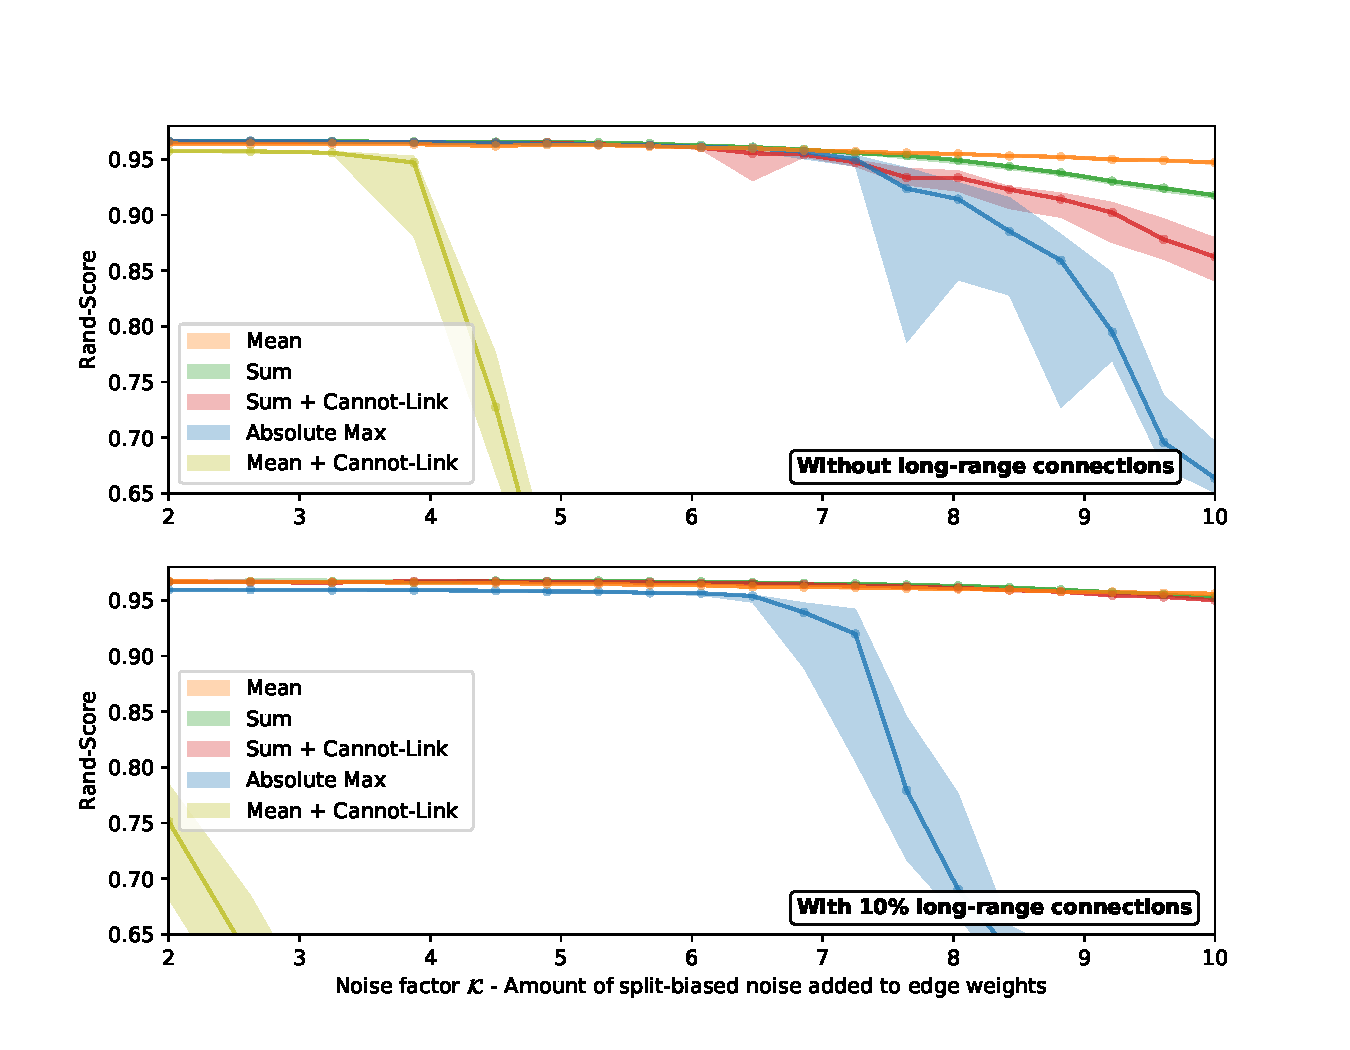
\includegraphics[width=0.98\textwidth,trim=0.29in 0.31in 0.31in 0.31in,clip]{./figs/split_noise.pdf}
        \caption{Split-biased opensimplex noise} \label{fig:ws}
    \end{subfigure}


\caption{Plot illustrating Adapted RAND scores achieved by UGACA and different update rules when noise is added to the edge weights... \TODO{Label which uses only local-neighbors and which uses long-range connections}}\label{fig:noise_merge}
\end{figure*}


\subsection{Noise experiments}
\begin{itemize}
    \item In this section we will quantitatively test the robustness of UGACA by adding noise to the edge weights of the graph and see how different choices of update rules compare.
    \item Among the update rules listed in Table \ref{tab:linkage-criteria}, we will focus only on \emph{sum}, \emph{arithmetic mean} and \emph{absolute maximum}, since they achieved the best scores in the results presented in Sec. \ref{sec:exp_first_comparison}. Before to present the results shown in Fig. \ref{fig:noise_merge}, we will first introduce the type of noise that was added to the edge weights.
\item In the set of experiments presented in this article, edge weights are estimated \UPDATE{by using a CNN that predicts how likely two neighboring pixels are to be part of the same cluster}. Fig. \ref{fig:noisy_affinities}a illustrates the predictions of the CNN. In image processing there are several ways of adding noise to an image, among which the most common are probably  for neighboring pixels in the horizontal direction of Define Perlin/opensimplex noise
\item Present plots
\item Comment about MC energy
\end{itemize}




% \begin{figure}
% \centering
% \includegraphics[width=0.50\textwidth,trim=0.27in 0.27in 0.27in 0.27in,clip]{./figs/noisy_affs.pdf}
% \caption{Illustration of noisy affinities}\label{fig:noisy_affinities}
% \end{figure}
